\documentclass{beamer}

\usepackage[labelformat=empty]{caption}

\mode<presentation>
{
  \usetheme{Berkeley}
  \usecolortheme{seagull}
  \setbeamercovered{transparent}
}

\title{Nuclear Energy is \\ important, old, new, and complicated}
\author{Jeffrey Seifried}
\institute{Ad Delivery Team, Yelp}
\date{Applied Learning Group, \texttt{2015-03-16}}

\AtBeginSubsection[]
{
  \begin{frame}<beamer>{Outline}
    \tableofcontents[currentsection,currentsubsection]
  \end{frame}
}


\begin{document}

\begin{frame}
  \titlepage
\end{frame}

\begin{frame}{Outline}
  \tableofcontents
\end{frame}


\section{About Me}

    \begin{frame}{1) Spend a decade in nuclear energy \\ 2) Data Miner at Yelp \; \; 3) ??? \; \; 4) Profit!}

        \begin{itemize}

            \item BSNE at University of Maryland, College Park
            \begin{itemize}
                \item Became a nuclear reactor operator
                \item Spent 4 summers + 1 semester \\ at the U.S. Nuclear Regulatory Commission
            \end{itemize}

            \pause

            \item PhDNE at UC, Berkeley and Lawrence Livermore Lab
            \begin{itemize}
                \item Developed reactor simulations
                \item Propagated uncertainties through them
                \item Helped design a hybrid fusion-fission reactor
            \end{itemize}

            \pause

            \item 2 year postdoc
            \begin{itemize}
                \item Developed reactor simulations
                \item Taught a course on nuclear reactor physics
                \item Helped design a thorium-fueled breed and burn reactor
            \end{itemize}
        \end{itemize}

    \end{frame}

\section{Nuclear energy}

    \subsection{... is important}

        \begin{frame}{``Dear future generations: Please accept our apologies, we were roaring drunk on petroleum.''}{- Kurt Vonnegut}

            \begin{itemize}

                \item Climate change is just getting ramped up
                \pause
                \item Coal particulates cause 10 thousand \\ deaths annually in the US
                \pause
                \item One quarter of California air pollution is from China
                \pause

                \vspace{2em}

                \item Global energy use will increase by a third by 2040
                \pause
                \item Natural gas and oil just got a lot cheaper
                \pause
                \item Coal is and always will be cheap

            \end{itemize}

        \end{frame}

        \begin{frame}{We need a scalable, baseload, carbon-free energy source.  Right now!}

            \begin{columns}[T]

                \begin{column}{0.5\textwidth}
                    \begin{figure}
                        \centering
                        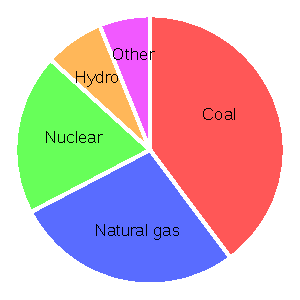
\includegraphics[width=\textwidth]{./img/sources.pdf}
                        \caption*{US elecriticity sources (2014)}
                    \end{figure}
                \end{column}

                \begin{column}{0.5\textwidth}
                    \begin{itemize}
                        \item Fossil Fuels generate 66\%
                        \pause
                        \item Nuclear generates 20\%
                        \pause
                        \item ... and 60\% of carbon-free electricity
                        \pause
                        \item Hydroelectric is shrinking
                        \pause
                        \item Renewables (``other'') are not ready
                    \end{itemize}
                \end{column}

            \end{columns}

        \end{frame}

    \subsection{... is old}

        \begin{frame}{The fission chain reaction \\ is at the heart of nuclear energy}

            \begin{columns}[T]

                \begin{column}{0.5\textwidth}
                    \begin{enumerate}
                        \item A neutron tickles a uranium nucleus
                        \pause
                        \item ... which splits into garbage, energy, and 2-3 neutrons
                        \pause
                        \item ... on average, 1-2 neutrons leak from the system or are consumed in a non-fission reaction
                        \pause
                        \item ... and 1 survives to cause another fission
                    \end{enumerate}
                \end{column}

                \begin{column}{0.5\textwidth}
                    \begin{figure}
                        \centering
                        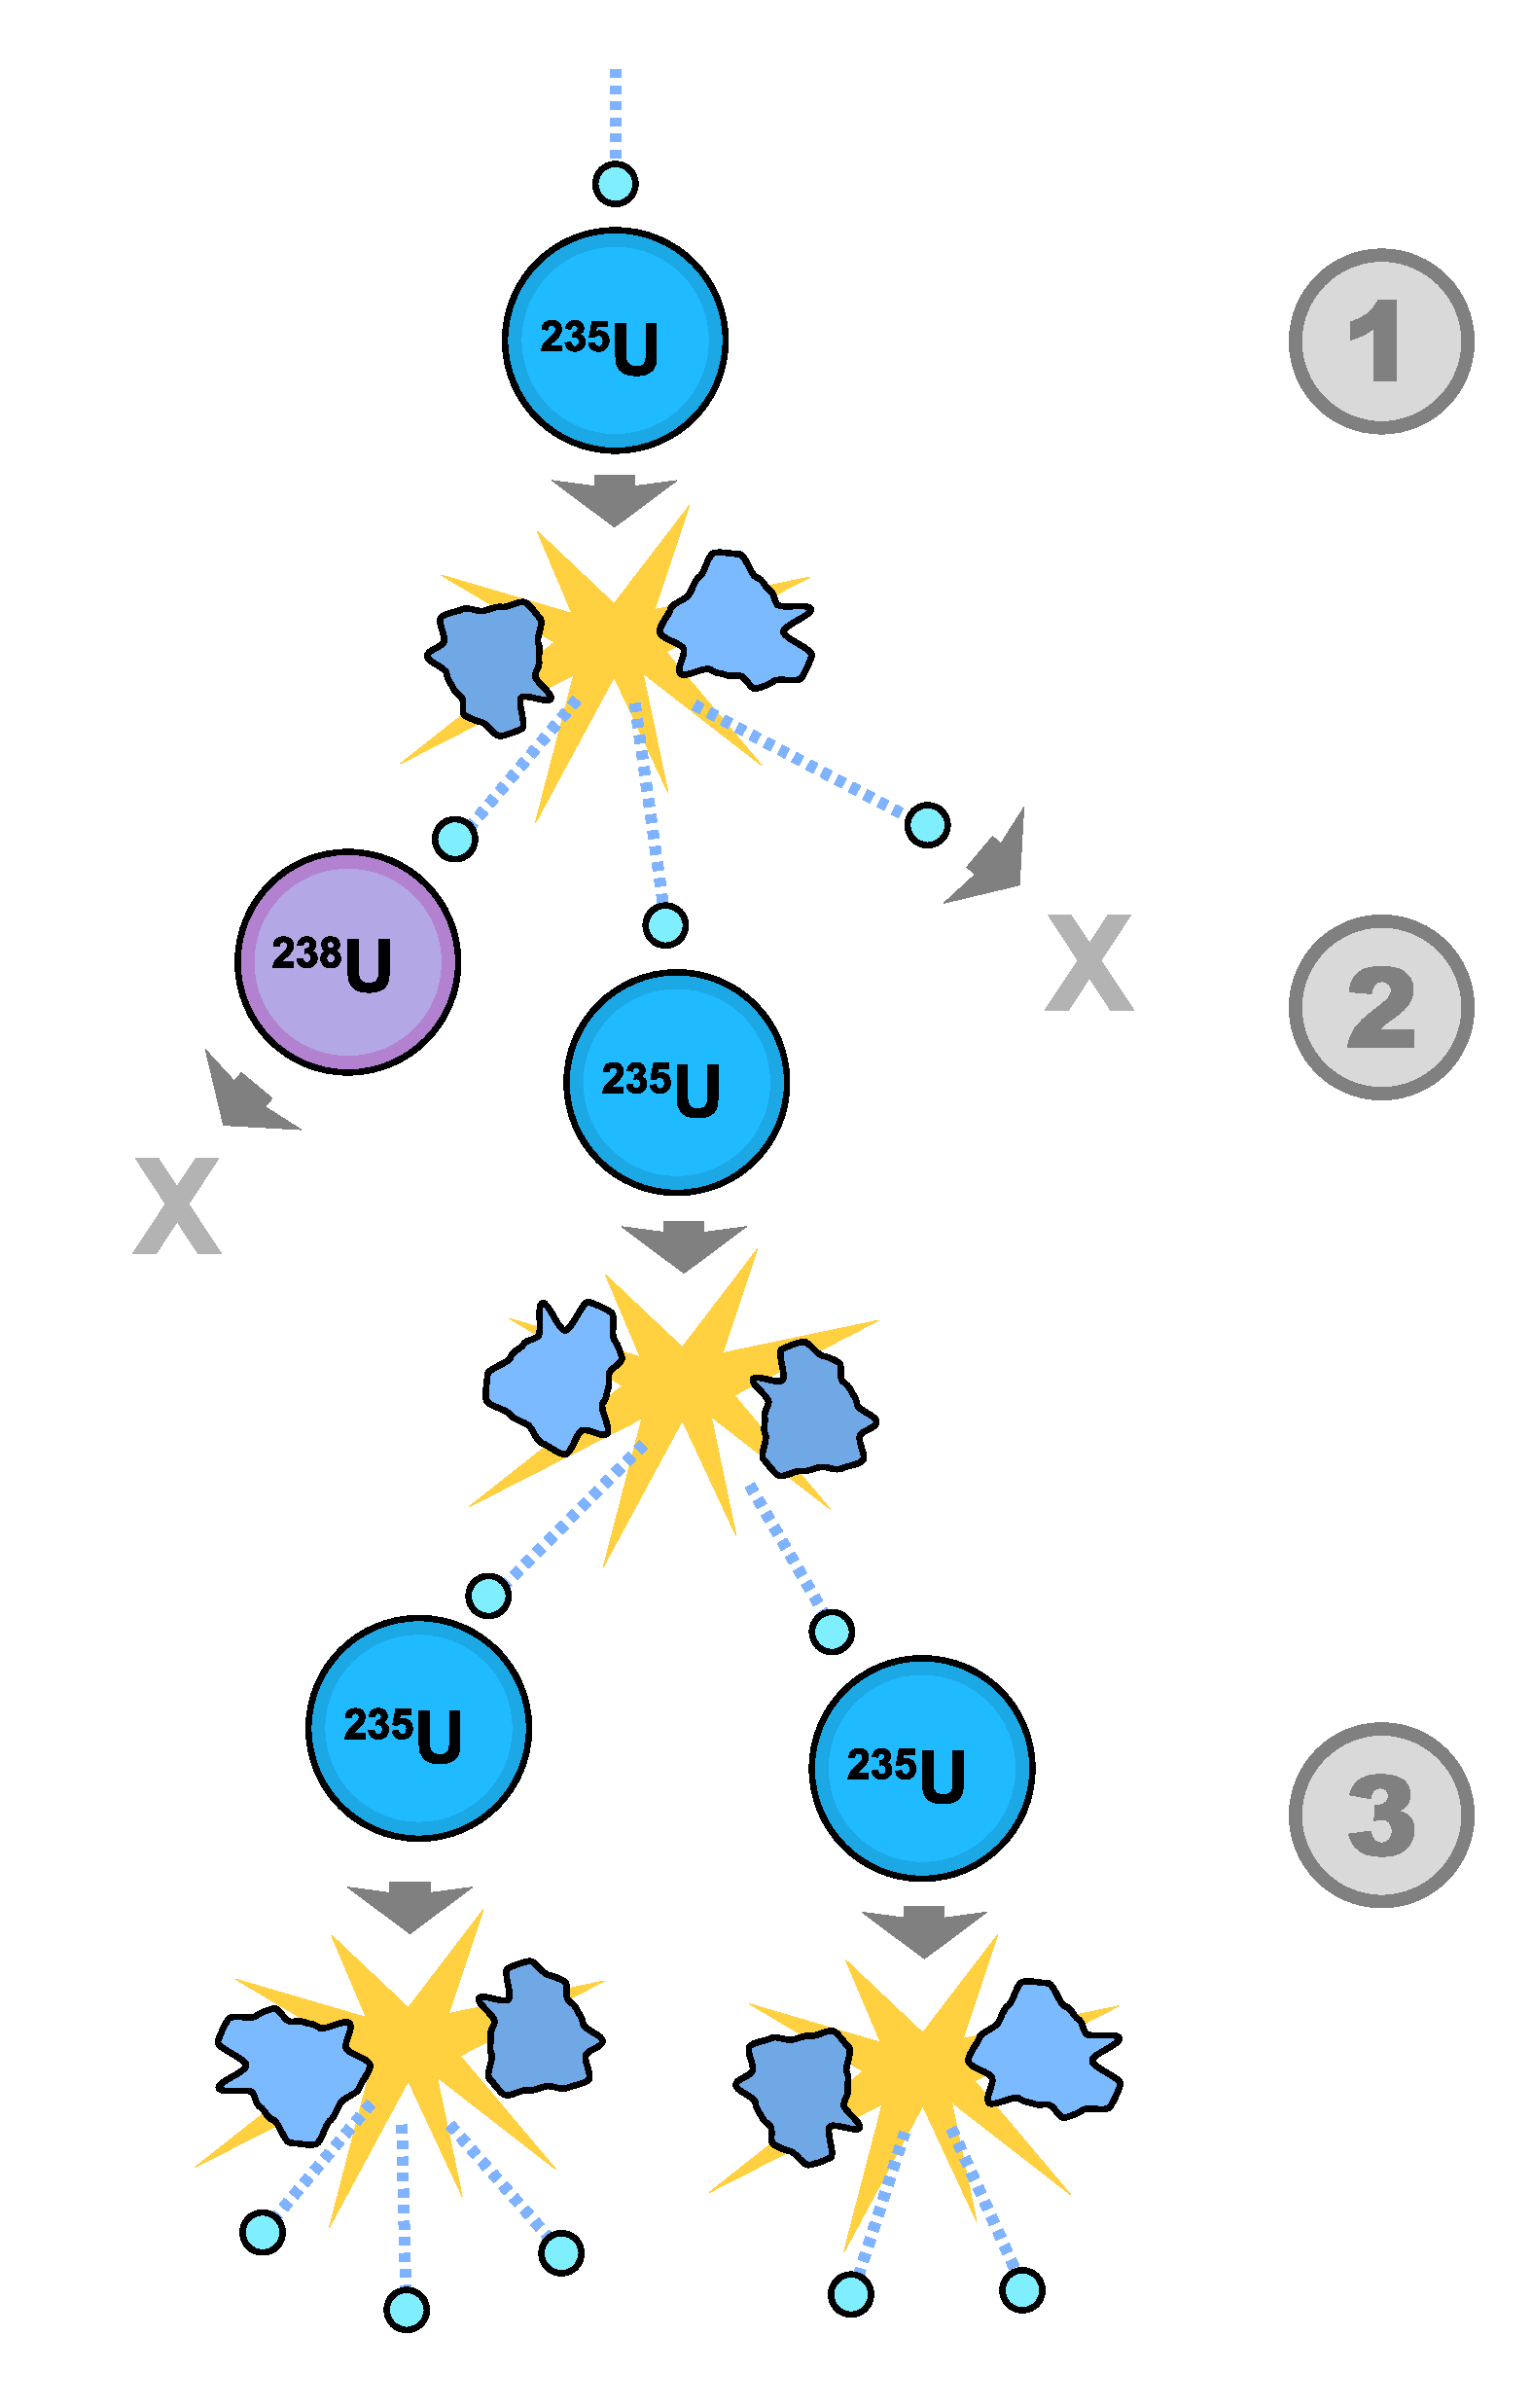
\includegraphics[width=0.7\textwidth]{./img/chainReaction.pdf}
                        \caption*{The fission chain reaction}
                    \end{figure}
                \end{column}

            \end{columns}

        \end{frame}

        \begin{frame}{The US nuclear fleet is composed of \\ roughly 100 light water reactors (LWR)}

            \begin{columns}[T]

                \begin{column}{0.5\textwidth}
                    \begin{figure}
                        \centering
                        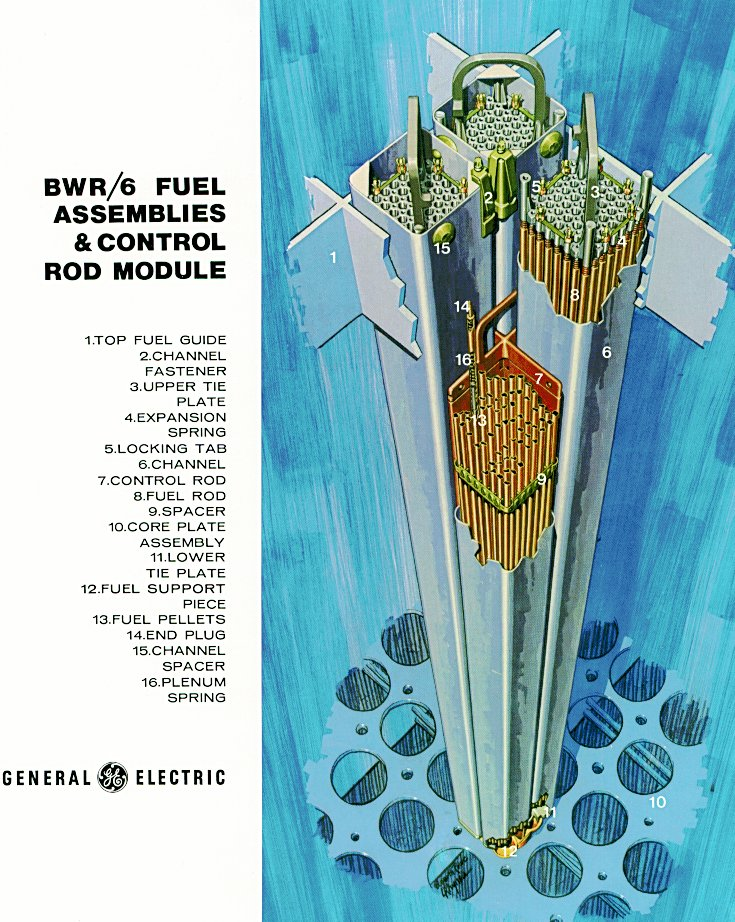
\includegraphics[width=0.8\textwidth]{./img/bwrFuel.png}
                        \caption*{An LWR fuel assembly}
                    \end{figure}
                \end{column}

                \begin{column}{0.5\textwidth}
                    \begin{figure}
                        \centering
                        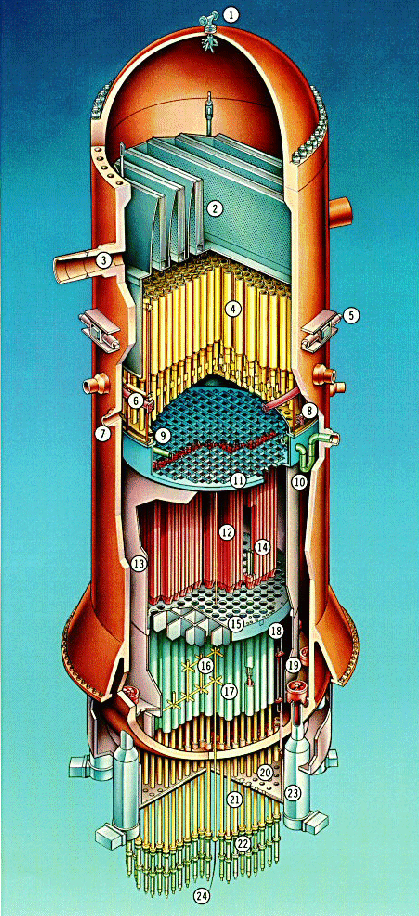
\includegraphics[width=0.5\textwidth]{./img/bwrCore.png}
                        \caption*{An LWR core}
                    \end{figure}
                \end{column}

            \end{columns}

        \end{frame}

        \begin{frame}{Nuclear reactors power 1800's era steam engines \\ just like coal, oil, and some natural gas}

            \begin{columns}[T]

                \begin{column}{0.5\textwidth}
                    \begin{figure}
                        \centering
                        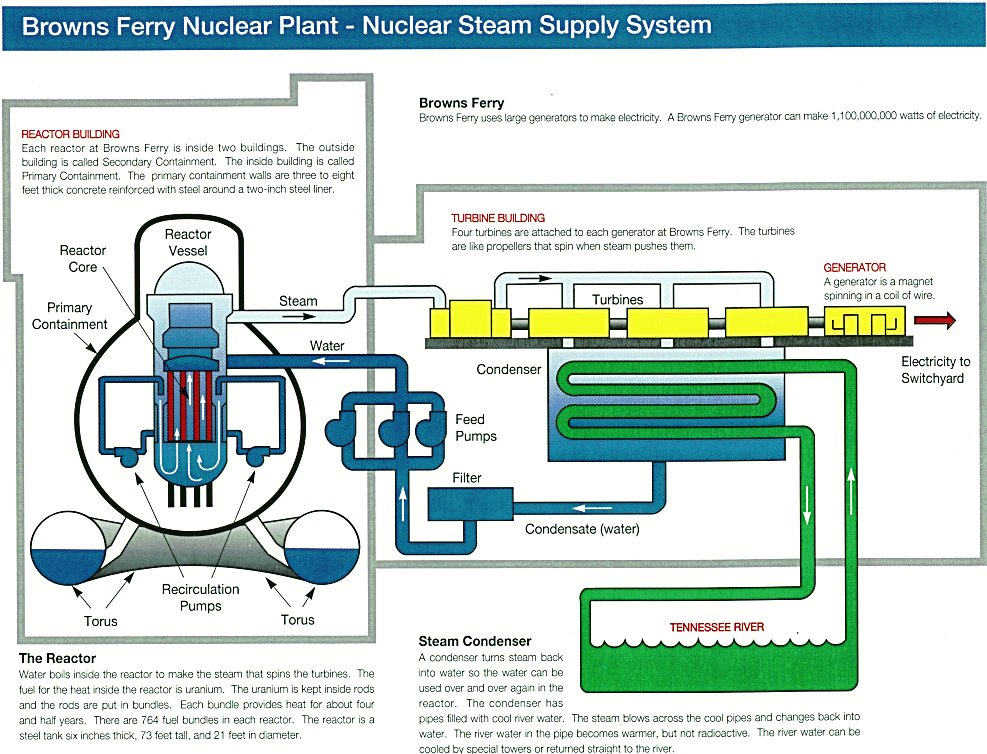
\includegraphics[width=\textwidth]{./img/bwrBop.png}
                        \caption*{Neutrons to electrons}
                    \end{figure}
                \end{column}

                \begin{column}{0.5\textwidth}
                    \begin{itemize}
                        \item Fission chain reaction releases heat
                        \pause
                        \item ... which boils water
                        \pause
                        \item ... which turns a turbine
                        \pause
                        \item ... which rotates a generator
                        \pause
                        \item ... which generates electricity!
                        \pause

                        \vspace{2em}

                        \item Only one third of heat energy is converted to electricity

                    \end{itemize}
                \end{column}

            \end{columns}

        \end{frame}

        \begin{frame}{We have come a long way since 1978}
            \begin{itemize}
                \item The most recent plant was built in 1996
                \pause
                \item ... its construction began in 1978
                \pause
                \item ... its design process took place in the early 1970's
            \end{itemize}
        \end{frame}

        \begin{frame}{There is room for improvement}
            \begin{itemize}
                \item Spent nuclear fuel is waiting for disposal
                \pause
                \item The core needs to be actively cooled
                \pause
                \item The fuel can melt
                \pause
                \item The water must be at high pressures
                \pause
                \item Two-thirds of energy is lost
            \end{itemize}
        \end{frame}

    \subsection{... is new}

        \begin{frame}{Sodium-cooled Fast reactors (SFR) consume nuclear waste, recycle it, and consume it again}
            \begin{figure}
                \centering
                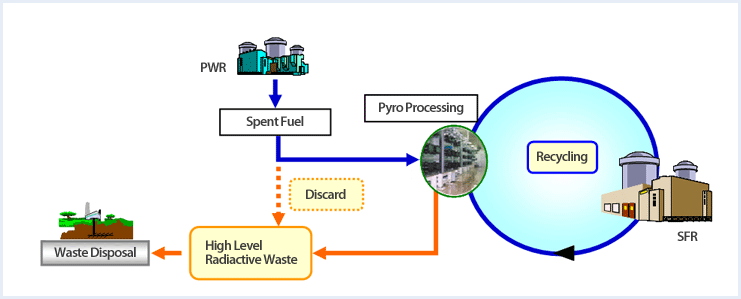
\includegraphics[width=1.0\textwidth]{./img/fastCycle.png}
                \caption*{}
            \end{figure}
        \end{frame}

        \begin{frame}{Traveling wave reactors (TWR; Breed \& Burn reactors) breed their own fuel without recycling}
            \begin{figure}
                \centering
                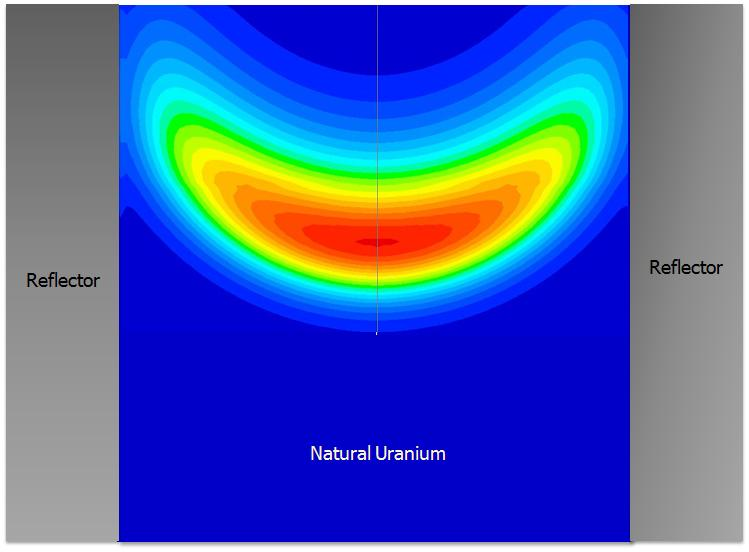
\includegraphics[width=0.9\textwidth]{./img/candle.png}
                \caption*{}
            \end{figure}
        \end{frame}

        \begin{frame}{Fluoride-salt high-temperature reactors (FHR) \\ can be passively cooled with ambient air}
            \begin{figure}
                \centering
                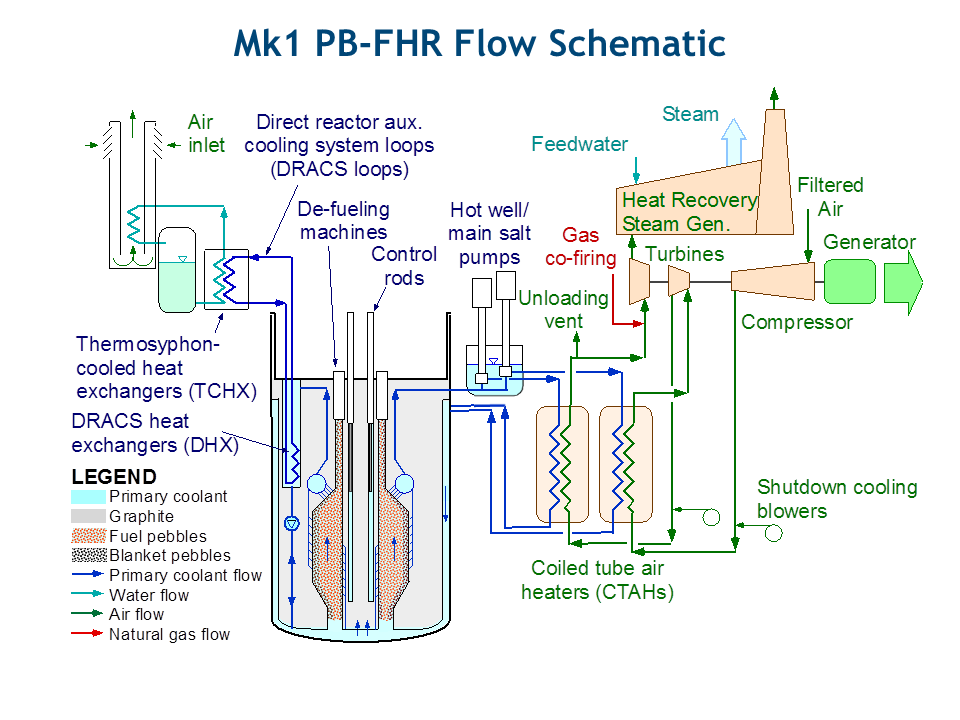
\includegraphics[width=0.9\textwidth]{./img/fhrBop.png}
                \caption*{}
            \end{figure}
        \end{frame}

        \begin{frame}{FHR's use coated particle fuel which cannot melt}
            \begin{figure}
                \centering
                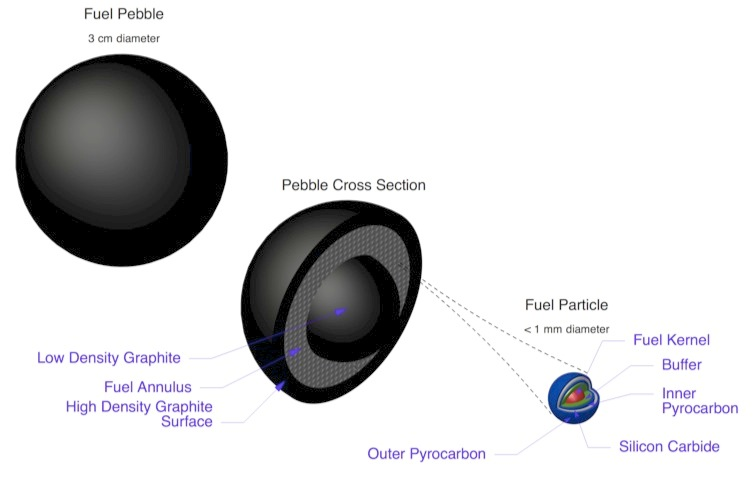
\includegraphics[width=1.0\textwidth]{./img/fhrPebble.png}
                \caption*{}
            \end{figure}
        \end{frame}

        \begin{frame}{FHR's replace water with fluoride salts \\ which boil at 1430$^{\circ}$C}
            \begin{figure}
                \centering
                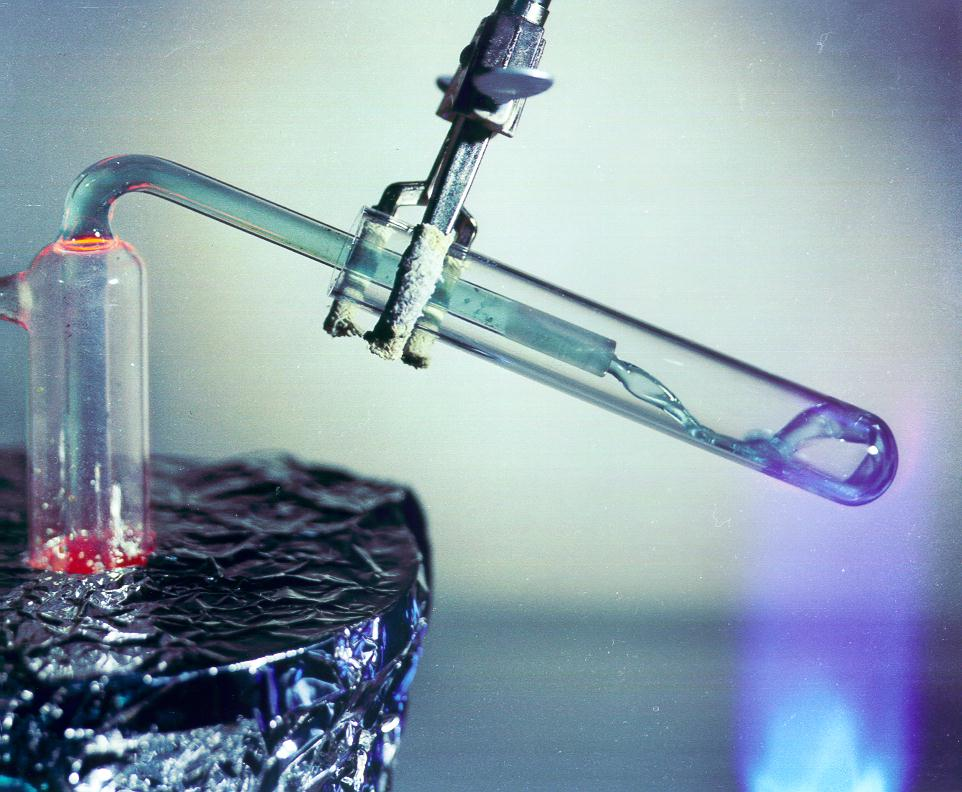
\includegraphics[width=0.8\textwidth]{./img/fhrFlibe.png}
                \caption*{}
            \end{figure}
        \end{frame}

        \begin{frame}{FHR's use modern air turbines \\ which are efficient and offer load following}
            \begin{figure}
                \centering
                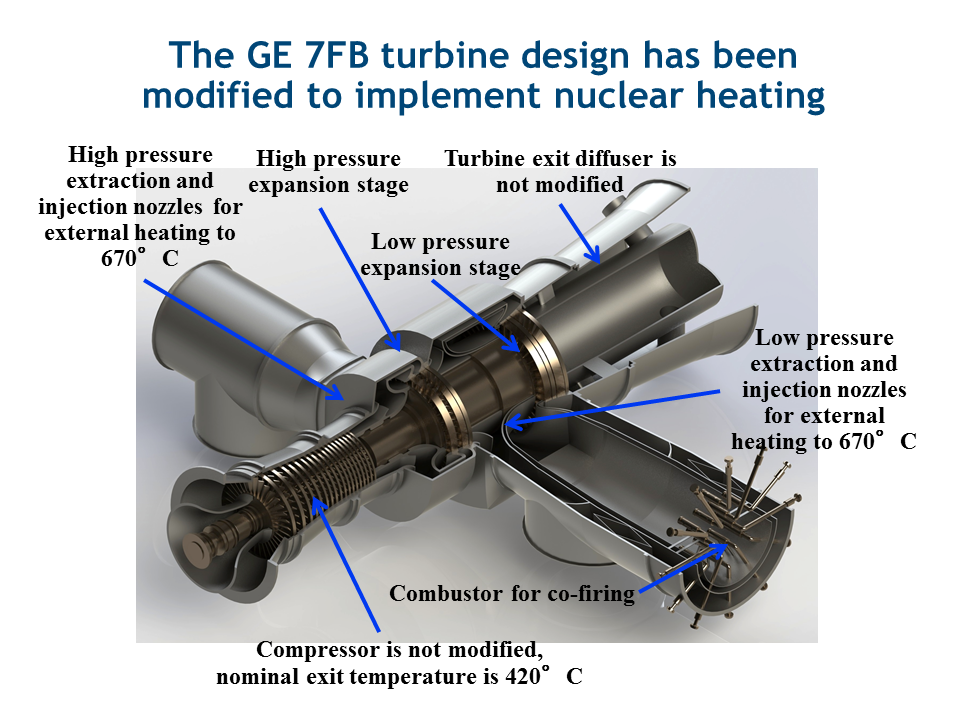
\includegraphics[width=0.9\textwidth]{./img/fhrPower.png}
                \caption*{}
            \end{figure}
        \end{frame}

        \begin{frame}{Fusion energy is star power on earth! \\ It produces no nuclear waste!}
            \begin{figure}
                \centering
                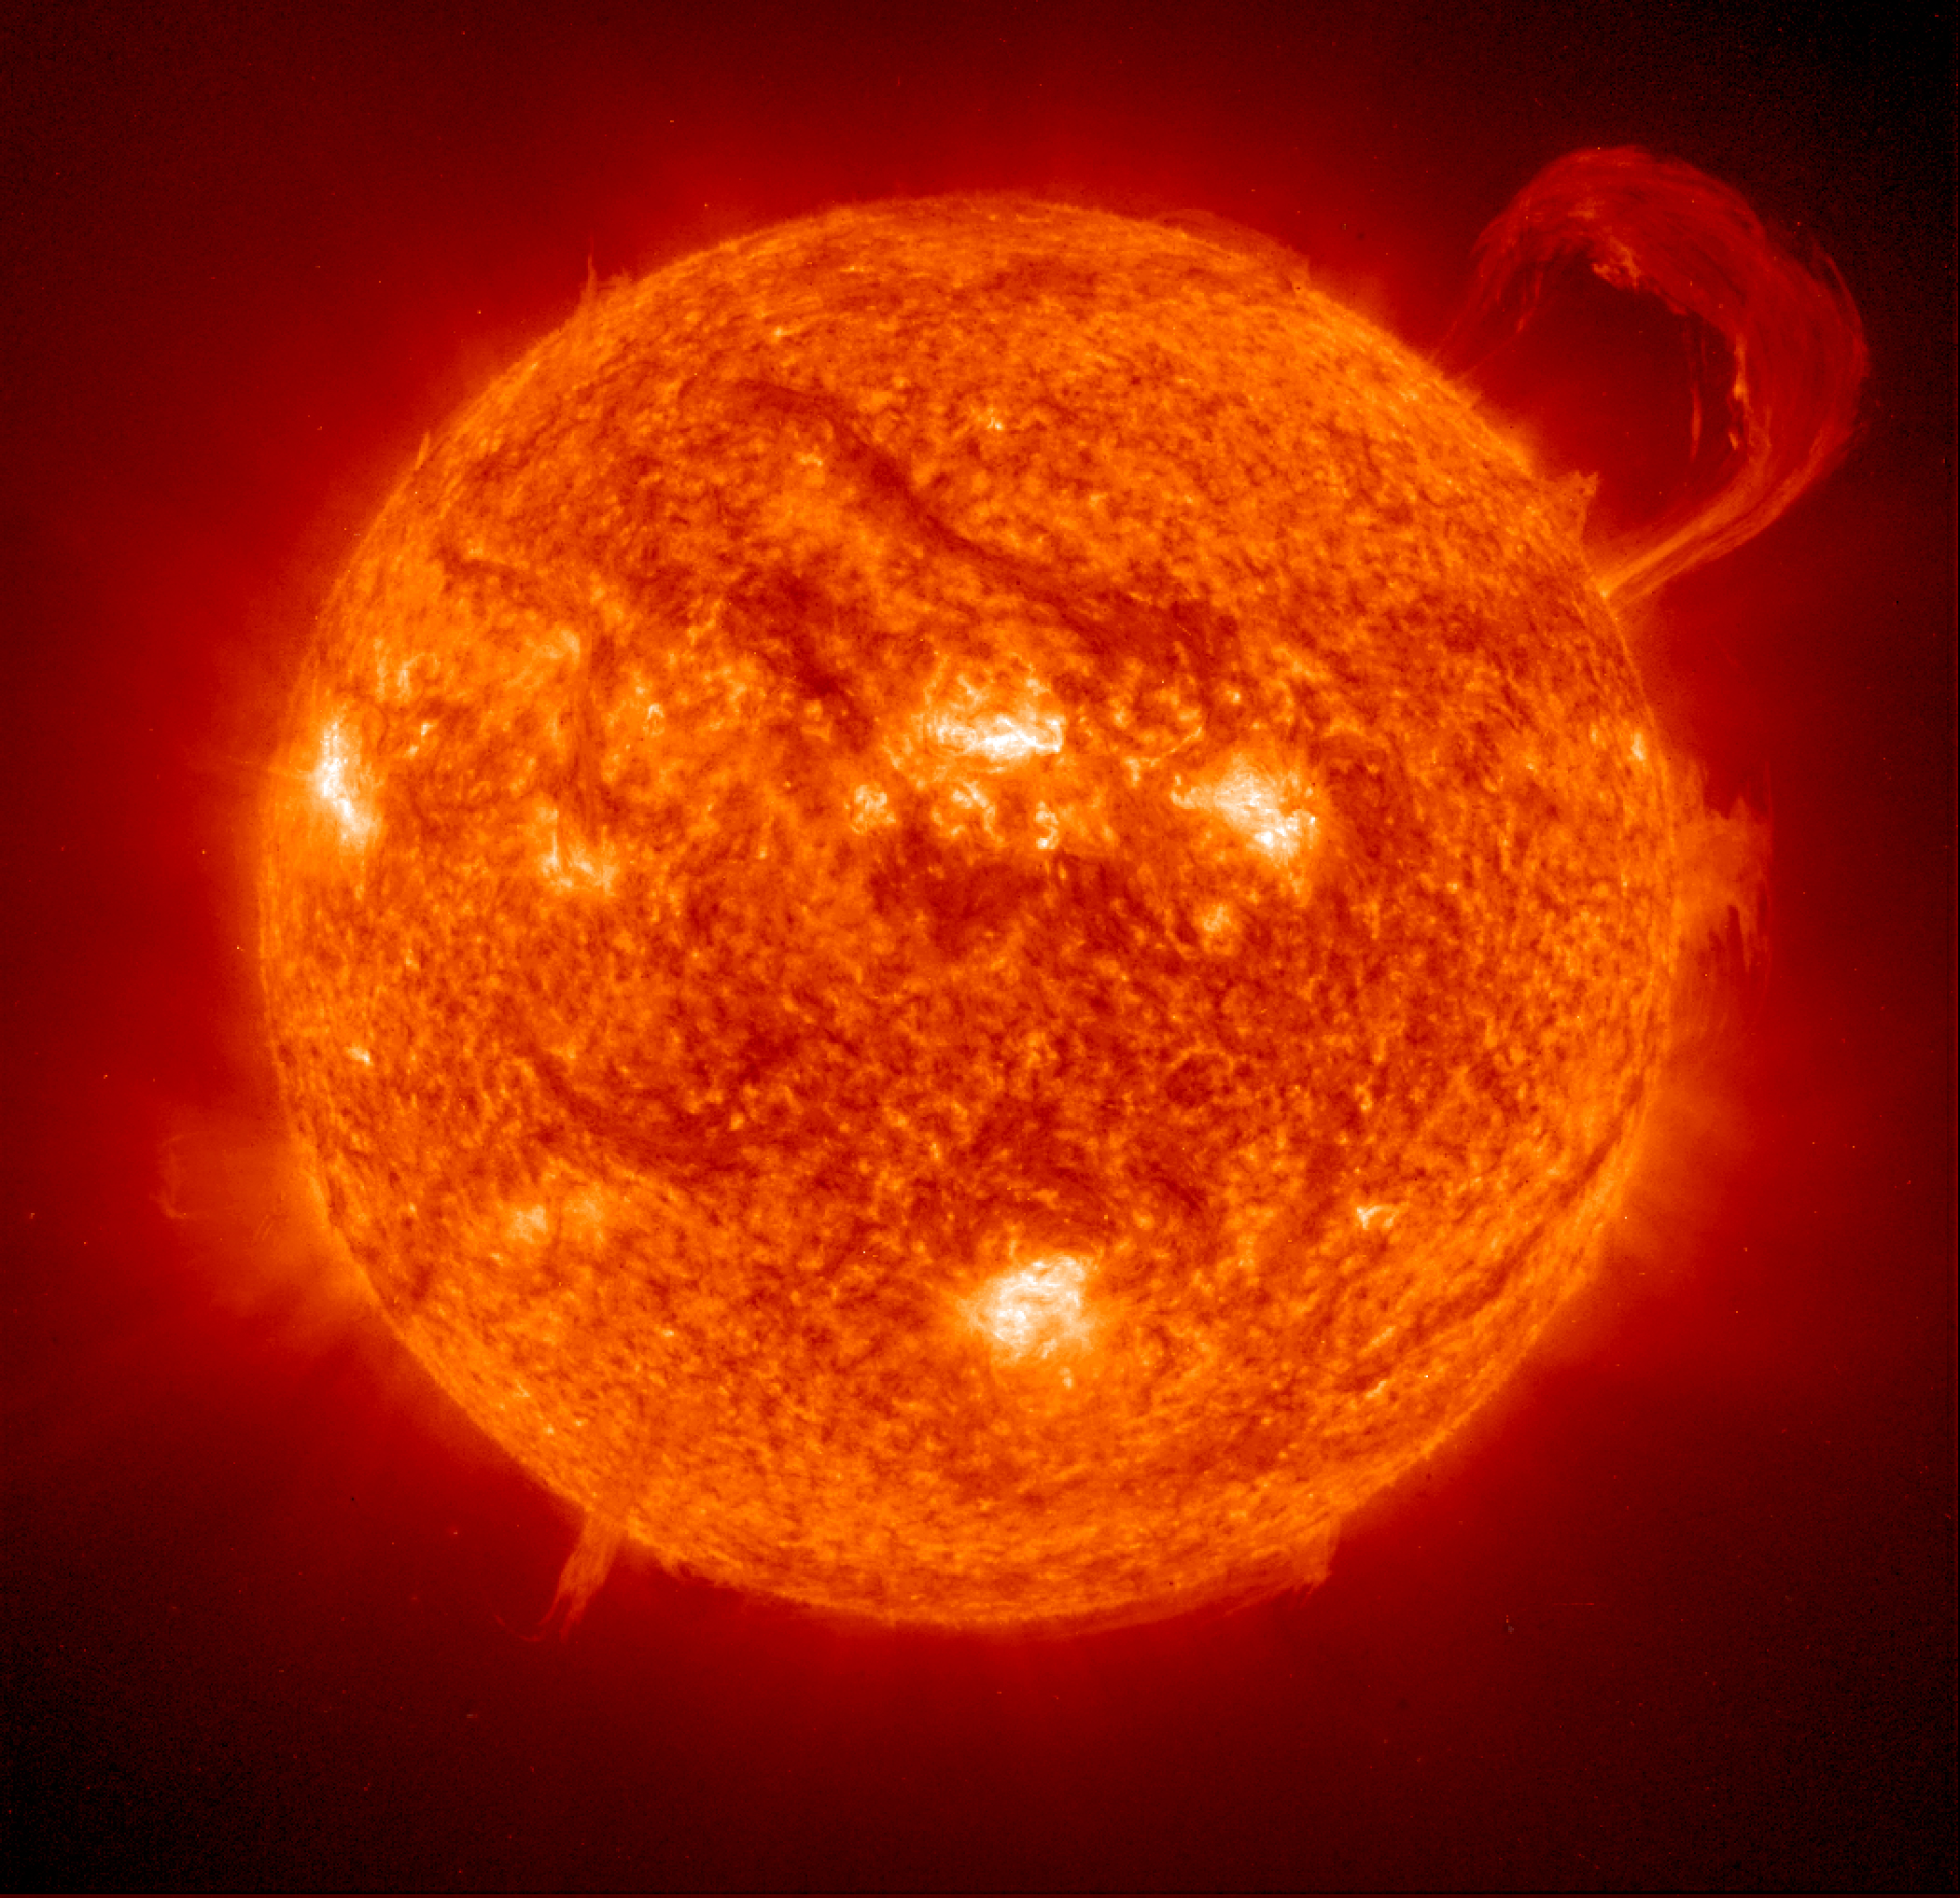
\includegraphics[width=0.7\textwidth]{./img/theSun.jpg}
                \caption*{}
            \end{figure}
        \end{frame}

        \begin{frame}{There is enough fusion fuel in the ocean to power humanity until the earth spins into the sun.}
            \begin{figure}
                \centering
                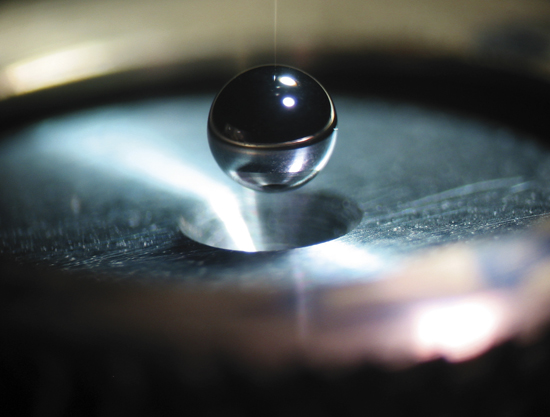
\includegraphics[width=0.9\textwidth]{./img/lifeFuel.png}
                \caption*{}
            \end{figure}
        \end{frame}

        \begin{frame}{However, controlled fusion is really difficult.  The NIF experiment at LLNL came close to break-even}
            \begin{figure}
                \centering
                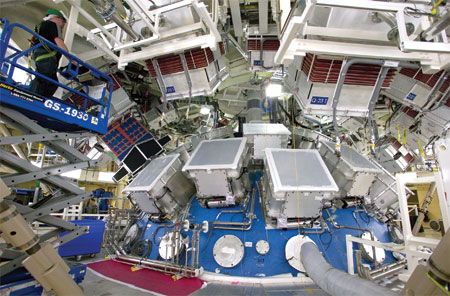
\includegraphics[width=1.0\textwidth]{./img/nifChamber.png}
                \caption*{}
            \end{figure}
        \end{frame}

        \begin{frame}{Hybrid fusion-fission reactors will be an economic stepping stone until fusion energy is perfected}
            \begin{figure}
                \centering
                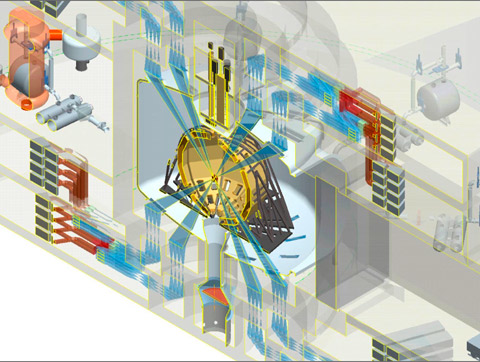
\includegraphics[width=0.9\textwidth]{./img/lifeChamber.png}
                \caption*{}
            \end{figure}
        \end{frame}

\section{Simulations}

    \subsection{The neutron transport equation}

        \begin{frame}{Accurate simulation of neutron fields requires their description 7-dimensional neutron phase space}
            \begin{figure}
                \centering
                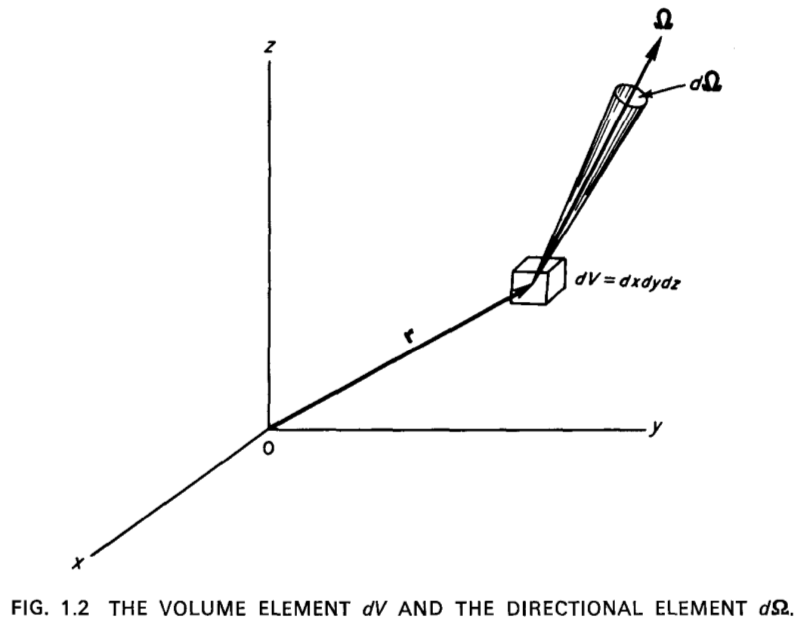
\includegraphics[width=0.9\textwidth]{./img/phaseSpace.png}
            \end{figure}
        \end{frame}

        \begin{frame}{Spatial distributions $(\vec r)$ can be complicated}
            \begin{figure}
                \centering
                
\includegraphics[width=0.7\textwidth]{./img/spaceFlux1.png}
                \caption*{}
            \end{figure}
        \end{frame}

        \begin{frame}{Spatial distributions $(\vec r)$ can be complicated}
            \begin{figure}
                \centering
                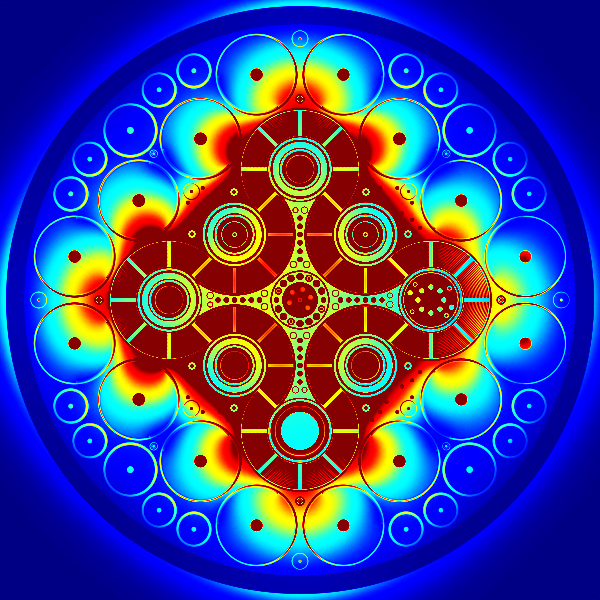
\includegraphics[width=0.7\textwidth]{./img/spaceFlux2.png}
                \caption*{}
            \end{figure}
        \end{frame}

        \begin{frame}{Spatial distributions $(\vec r)$ can be complicated}
            \begin{figure}
                \centering
                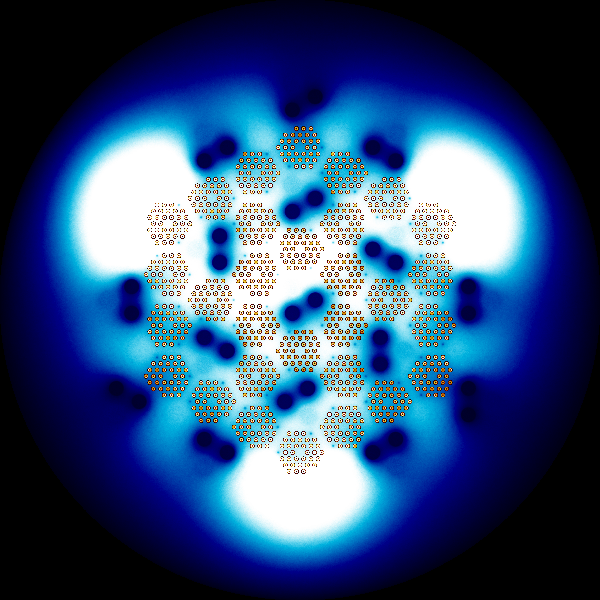
\includegraphics[width=0.7\textwidth]{./img/spaceFlux3.png}
                \caption*{}
            \end{figure}
        \end{frame}

        \begin{frame}{Energy distributions $(E)$ can be complicated}
            \begin{figure}
                \centering
                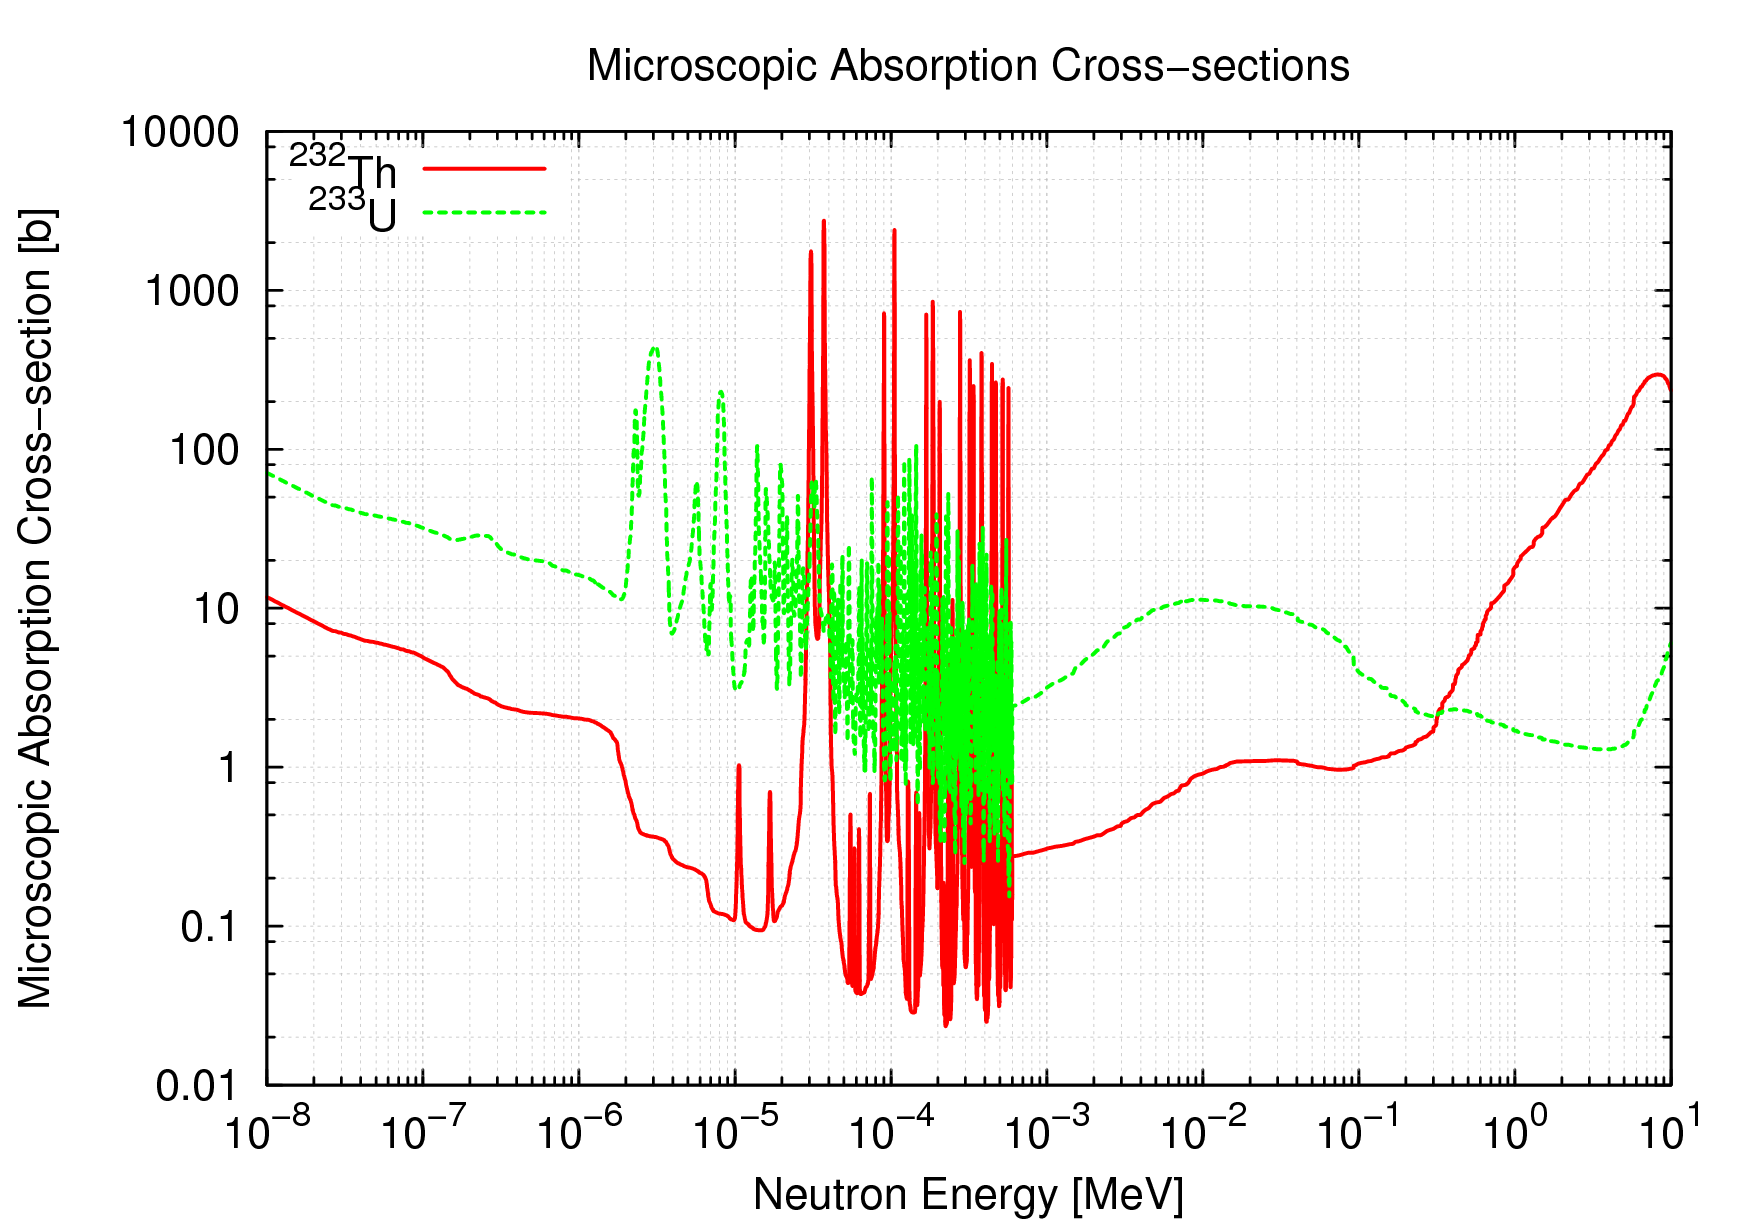
\includegraphics[width=1.0\textwidth]{./img/energyXs.png}
                \caption*{}
            \end{figure}
        \end{frame}

        \begin{frame}{Energy distributions $(E)$ can be complicated}
            \begin{figure}
                \centering
                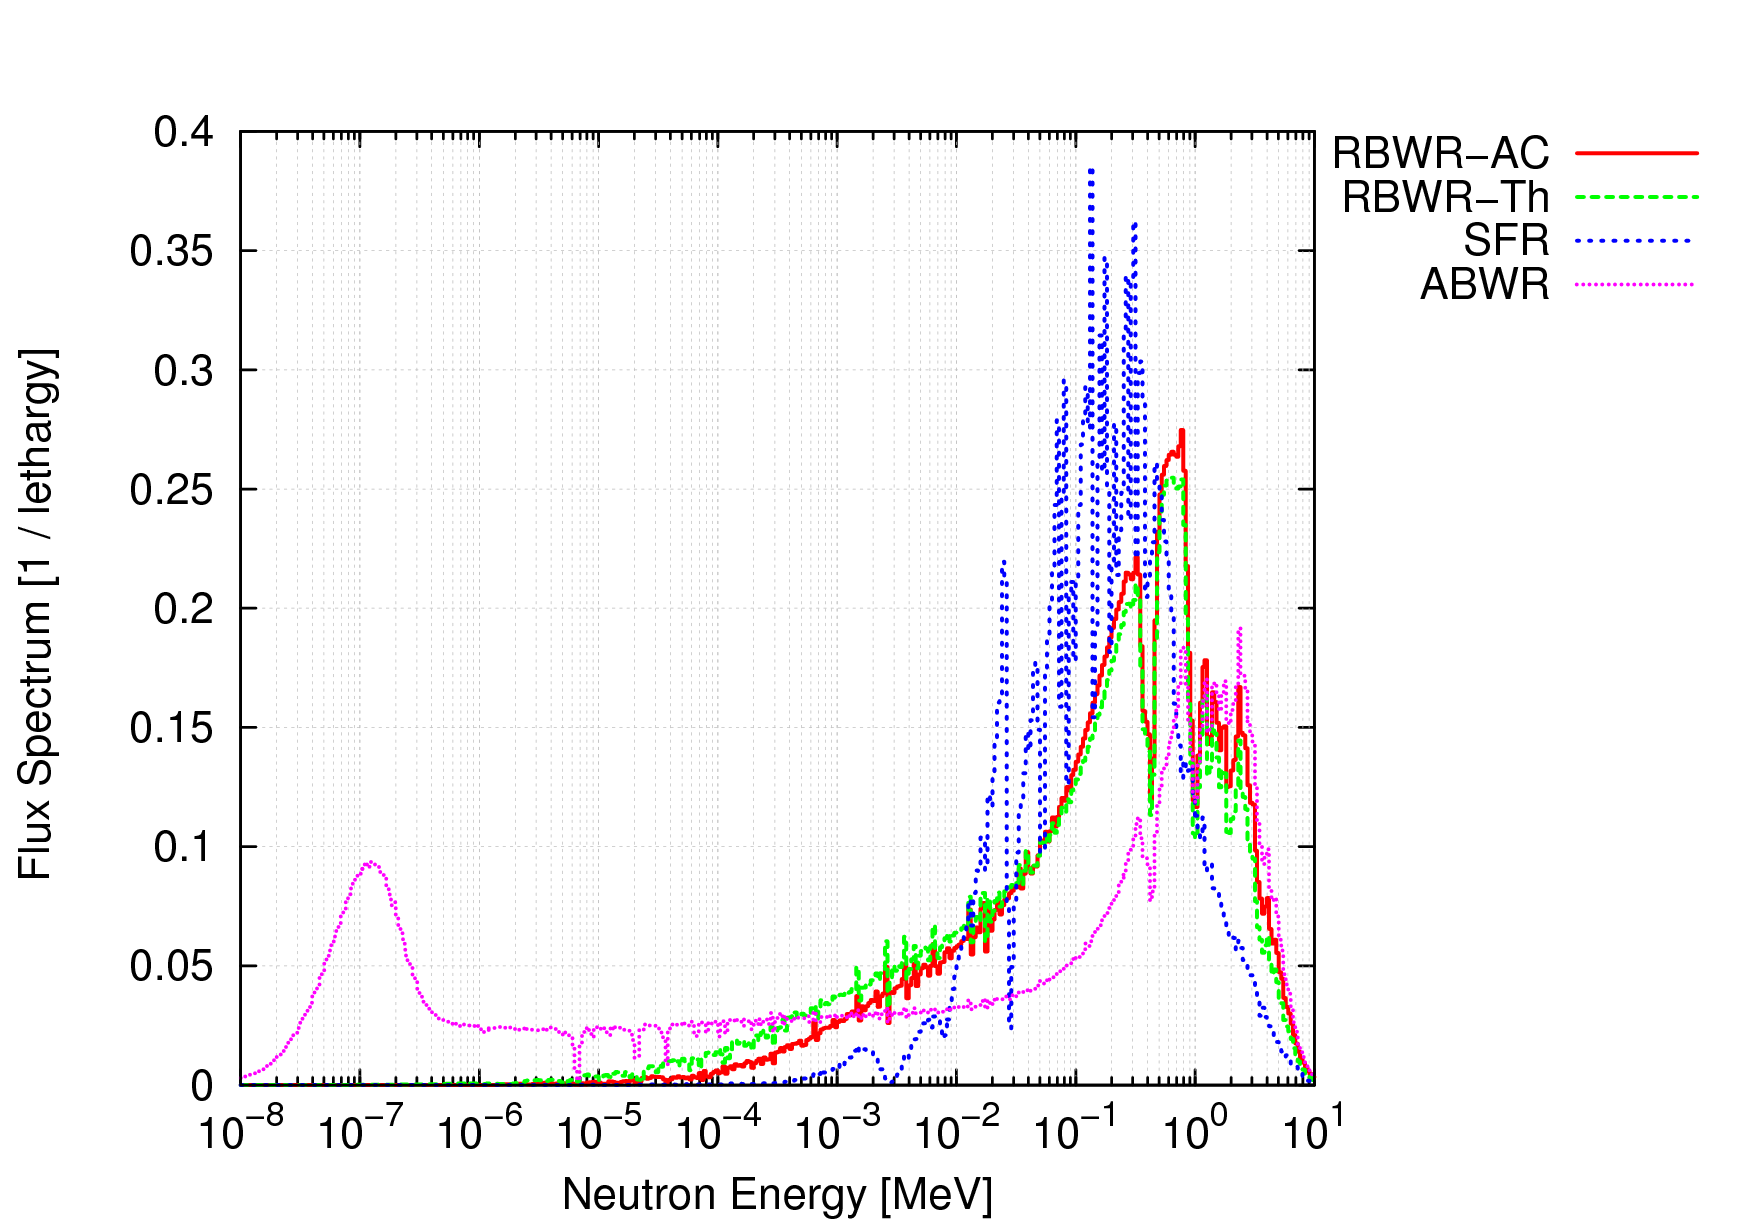
\includegraphics[width=1.0\textwidth]{./img/energyFlux.png}
                \caption*{}
            \end{figure}
        \end{frame}

        \begin{frame}{The neutron transport equation (NTE) balances sources and sinks within neutron phase space}
            \begin{equation*}
                \begin{split}
                    \vec \Omega \cdot \vec \bigtriangledown \; \; \psi(\vec r, E, \vec \Omega) \\
                    + \sigma_{total}(\vec r, E) \; \; N(\vec r) \; \; \psi(\vec r, E, \vec\Omega) \\
                    = \int_0^\infty \! \! \! \! dE \int_{4\pi} \! \! \! \! d\vec\Omega \; \; \sigma_{scatter}(\vec r, E^\prime \rightarrow E, \vec \Omega^\prime \cdot \vec \Omega) \; \; N(\vec r) \; \; \psi(\vec r, E^\prime, \vec\Omega^\prime) \\
                    + \frac{\chi(E)}{4\pi} \int_0^\infty \! \! \! \! dE^{\prime\prime} \; \; \nu (E^{\prime\prime}) \; \; \sigma_{fission}(\vec r, E^{\prime\prime}) \; \; N(\vec r) \; \; \psi(\vec r, E^{\prime\prime}, \vec\Omega^{\prime\prime}) \\
                    + \mathcal{S}_{ext}(\vec r, E, \vec\Omega)
                \end{split}
            \end{equation*}
        \end{frame}

        \begin{frame}{The easiest approach is simplification}
            \begin{itemize}
                \item Ignore energy dependence
                \pause
                \item Assume directional dependence is isotropic or linearly anisotropic
                \pause
                \item Approximate the system as a smeared homogeneous lump
                \pause
                \item Assume the spatial/spectral/directional dependencies are separable
                      (e.g., $\psi(\vec r, E, \vec\Omega) = \mathcal{R}(\vec r)\mathcal{E}(r)\mathcal{W}(\vec\Omega)$)
                      and solve them independently
                \pause

                \vspace{2em}

                \item You can get creative!
                \pause
                \item Also, garbage in, garbage out!
            \end{itemize}
        \end{frame}

        \begin{frame}{The next approach is discretization}
            \begin{enumerate}
                \item Divide spatial regions into cubes or tetrahedra, with interfaces
                \pause
                \item Divide the energy axis into hundreds or thousands of bins
                \pause
                \item Expand directional dependence in spherical harmonics
                \pause
                \item Consider at pseudo-steady-state snapshots in time
                \pause
                \item Write an enormous linear system and iterate until convergence
                \pause
                \item Sweep through the solution in a manner which mimics the physical path of neutrons
            \end{enumerate}
        \end{frame}

        \begin{frame}{The accurate approach is Monte Carlo neutron transport -- following neutrons one-at-a-time}
            \begin{enumerate}
                \item Assume a source distribution
                \pause
                \item Sample a neutron from it ($\vec r$, $E$, $\vec\Omega$)
                \pause
                \item Sample how far the neutron travels before a leak or collision
                \pause
                \item Sample the collision type (e.g., scatter, fission, capture)
                \pause
                \item Sample the collision outcome ($\vec r$, $E$, $\vec\Omega$)
                \pause
                \item Iterate until the source distribution converges
                \pause
                \item Consider accelerating with the simpler models above
            \end{enumerate}
        \end{frame}

        \begin{frame}{The NTE often depends upon other fields, so models need to be solved simultaneously}
            \begin{itemize}
                \item Fluids flow (Navier-Stokes)
                \pause
                \item Heat spreads (heat equation) and expands things (equation of state of the material)
                \pause
                \item Boiling water behaves differently from liquid water (closure relations)
                \pause
                \item Solve each one independently  -- holding the rest constant -- and iterate!
                \pause
                \item Choose a smart path and consider relaxation for acceleration or stability
            \end{itemize}
        \end{frame}

    \subsection{The Bateman equations}

        \begin{frame}{Isotope depletion, breeding, and decay can be complicated}
            \begin{figure}
                \centering
                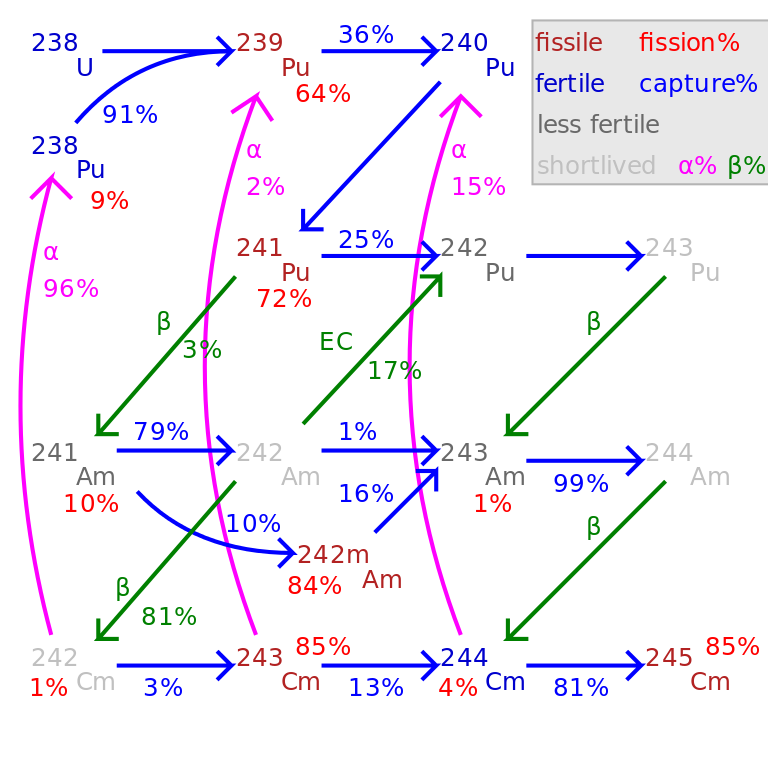
\includegraphics[width=0.7\textwidth]{./img/fuelCycle.png}
                \caption*{}
            \end{figure}
        \end{frame}

        \begin{frame}{The Bateman equations describe the time-evolution of isotopes during decay and irradiation}
            \begin{equation*}
                \begin{split}
                    \frac{\partial N_i(\vec r, t)}{\partial t} \\
                    + \lambda_i \; \; N_i(\vec r, t) \\
                    + \int_0^\infty \! \! \! \! dE \; \; \sigma_{absorption,i} ( \vec r, E) \; \; \int_{4\pi} \! \! \! \! d\vec\Omega \; \; \psi(\vec r, E, \vec \Omega) \; \; N_i(\vec r, t) \\
                    = \sum_j \left[ b_{j \rightarrow i} \; \; \lambda_j \; \; N_j(\vec r, t) \right] \\
                    + \sum_k \left[ b_{k \rightarrow i} \int_0^\infty \! \! \! \! dE \; \; \sigma_{absorption,k} ( \vec r, E) \; \; \int_{4\pi} \! \! \! \! d\vec\Omega \; \; \psi(\vec r, E, \vec \Omega) \; \; N_k(\vec r, t) \right] \\
                \end{split}
            \end{equation*}
        \end{frame}

        \begin{frame}{If you take the Laplacian \\ an analytical solution exists!}

            \begin{equation*}
                N_n(t) = \Pi_{j=1}^{n-1} \lambda_j \sum_{i=1}^n \sum_{j=1}^n \left(\frac{N_i(0) e^{-\lambda_j t}}{\Pi_{p=i,p\ne j}(\lambda_p - \lambda_j}\right)
            \end{equation*}

            \begin{itemize}
                \pause
                \item The formulation is numerically unstable in real cases
                \pause
                \item So, on practice, it is solved numerically
            \end{itemize}
        \end{frame}

        \begin{frame}{The ODE is homogeneous \\ so it can be written as a linear system}

            \begin{equation*}
                \frac{\partial\vec N}{\partial t} = \mathbb{T} \vec N
            \end{equation*}

            \begin{equation*}
                \vec N(t) = \vec N_0 e^{\mathbb{T} t}
            \end{equation*}

            \begin{equation*}
                \vec N(t) \approx \mathbb{I} + \mathbb{T}t + \frac{\left(\mathbb{T}t\right)^2}{2!} + \dots
            \end{equation*}

            \begin{itemize}
                \pause
                \item $\mathbb{T}$ is large and ill-conditioned in real cases
                \pause
                \item So, in practice many of the less relevant terms are zeroed and collapsed
            \end{itemize}
        \end{frame}

\section*{Summary}

    \begin{frame}{Nuclear energy is}
        \begin{itemize}
            \item ... important
            \pause
            \item ... old
            \pause
            \item ... new
            \pause
            \item ... complicated
        \end{itemize}
    \end{frame}

    \begin{frame}{Thank you!}
        \begin{figure}
            \centering
            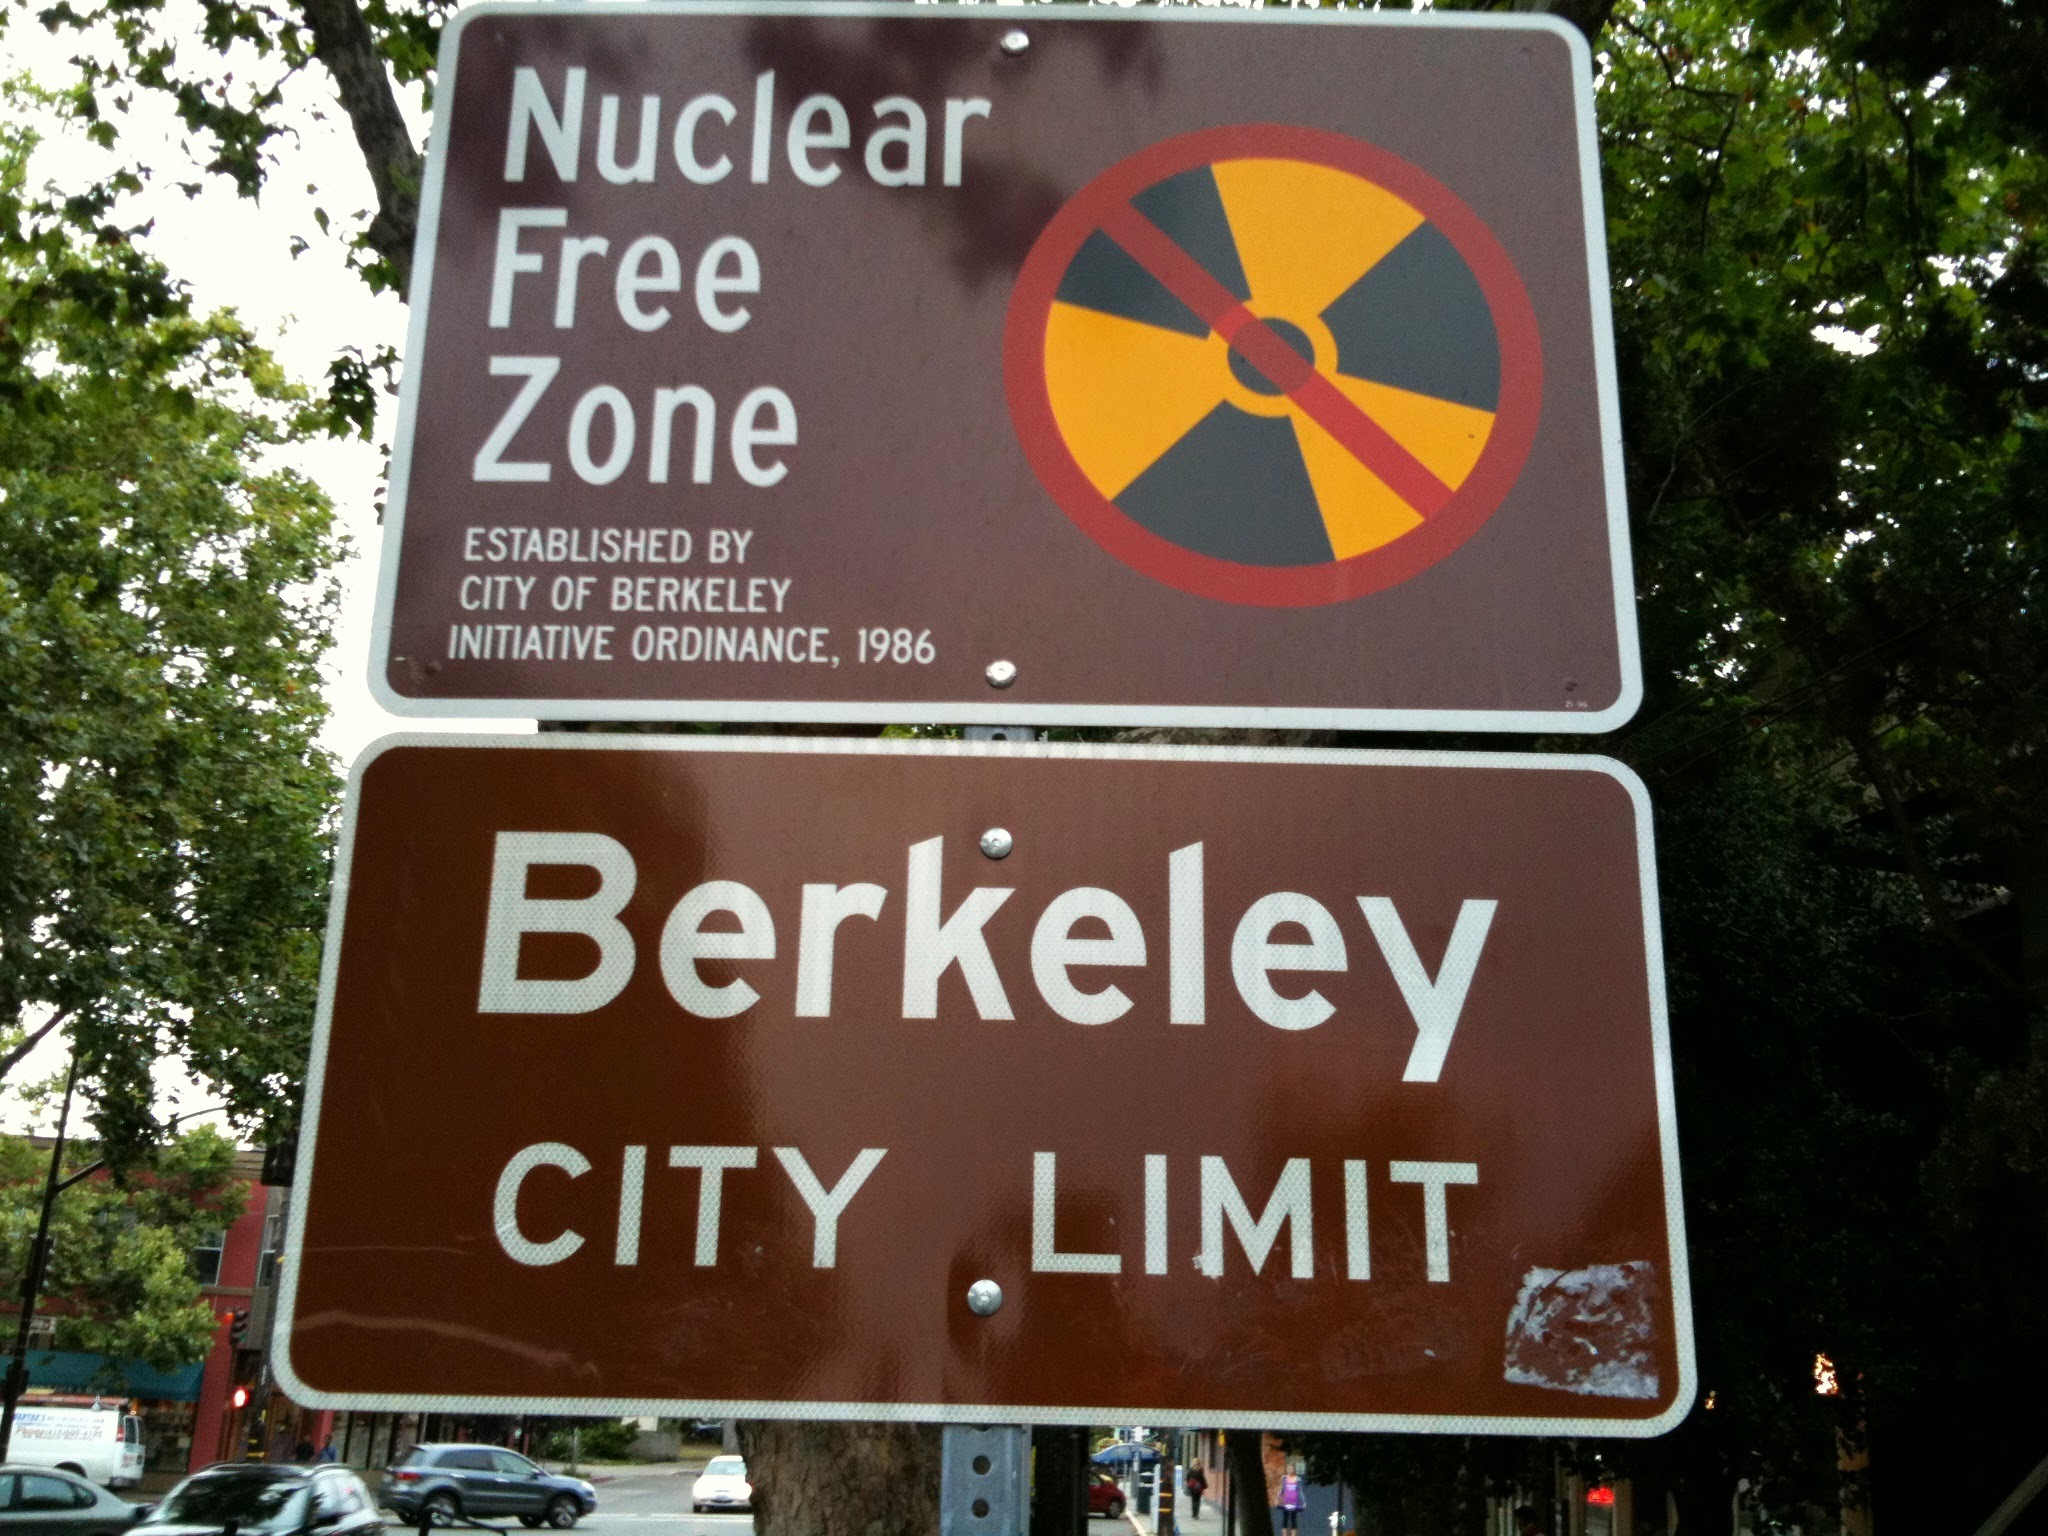
\includegraphics[width=0.9\textwidth]{./img/nuclearFree.jpg}
            \caption*{}
        \end{figure}
    \end{frame}

\end{document}
